%%%%%%%%%%%%%%%%%%%%%%%%%%%%%%%%%%%%%%%%%%%%%%%%%%%%%%%%%%%%
%%% ELIFE ARTICLE TEMPLATE
%%%%%%%%%%%%%%%%%%%%%%%%%%%%%%%%%%%%%%%%%%%%%%%%%%%%%%%%%%%%
%%% PREAMBLE 
\documentclass[9pt,lineno]{elife}
% Use the onehalfspacing option for 1.5 line spacing
% Use the doublespacing option for 2.0 line spacing
% Please note that these options may affect formatting.
% Additionally, the use of the \newcommand function should be limited.

%\newcommand{\pKa}{p$K_\mathrm{a}$}
\newcommand{\pKa}{pKa}

\usepackage{lipsum} % Required to insert dummy text
\usepackage[version=4]{mhchem}
\usepackage{siunitx}
\DeclareSIUnit\Molar{M}
\usepackage[colorinlistoftodos]{todonotes}
\usepackage{gensymb}
\usepackage{mhchem}

%%%%%%%%%%%%%%%%%%%%%%%%%%%%%%%%%%%%%%%%%%%%%%%%%%%%%%%%%%%%
%%% ARTICLE SETUP
%%%%%%%%%%%%%%%%%%%%%%%%%%%%%%%%%%%%%%%%%%%%%%%%%%%%%%%%%%%%
\title{pKa measurements for the SAMPL6 prediction challenge for a set of kinase inhibitor-like fragments
}

\author[1,2]{Mehtap Işık}
\author[3]{Dorothy Levorse}
\author[1,4]{Ari\"{e}n S. Rustenburg}
\author[5]{Ikenna Ndukwe}
\author[5]{Heather Wang}
\author[6]{David Mobley}
\author[3]{Timothy Rhodes}
\author[1*]{John D. Chodera}

\affil[1]{Computational and Systems Biology Program, Sloan Kettering Institute, Memorial Sloan Kettering Cancer Center, New York, NY 10065, United States}
\affil[2]{Tri-Institutional PhD Program in Chemical Biology, Weill Cornell Graduate School of Medical Sciences, Cornell University, New York, NY 10065, United States}
\affil[3]{Merck \& Co., Inc., MRL, Pharmaceutical Sciences, 126 East Lincoln Avenue, Rahway, New Jersey 07065, United States}
\affil[4]{Graduate Program in Physiology, Biophysics, and Systems Biology, Weill Cornell Medical College, New York, NY 10065, United States}
\affil[5]{Merck  Co., Inc., MRL, Process Research \& Development, 126 East Lincoln Avenue, Rahway, New Jersey 07065, United States}
\affil[6]{Department of Pharmaceutical Sciences and Department of Chemistry, University of California,
Irvine, Irvine, California 92697, United States}
\corr{john.chodera@choderalab.org}{JDC}

%%%%%%%%%%%%%%%%%%%%%%%%%%%%%%%%%%%%%%%%%%%%%%%%%%%%%%%%%%%%
%%% ARTICLE START
%%%%%%%%%%%%%%%%%%%%%%%%%%%%%%%%%%%%%%%%%%%%%%%%%%%%%%%%%%%%

\begin{document}

\maketitle

%%%%%%%%%%%%%%%%%%%%%%%%%%%%%%%%%%%%%%%%%%%%%%%%%%%%%%%%%%%%
% Abstract
%%%%%%%%%%%%%%%%%%%%%%%%%%%%%%%%%%%%%%%%%%%%%%%%%%%%%%%%%%%%
\begin{abstract}
Determining the protonation state of a small molecule is a preliminary requirement for predicting its physicochemical and pharmaceutical properties, as well as interactions with protein targets using computational models. To determine the ionic state of a molecule in an aqueous solution at a certain pH it is necessary to know its acid dissociation constants(pKas). As a part of SAMPL6 community challenge, we organized a blind pKa prediction component to asses the accuracy of contemporary pKa prediction methods. While inaccuracy in prediction of small molecule pKas have potential detrimental impact on predictive physical models, predicting pKas of drug-like molecules can be difficult due to challenging properties such as multiple titratable sites, heterocycles, and tautomerization. We limited the focus of this challenge on a subset of chemical space of drug-like molecules:  24 small molecules were selected to represent fragments of kinase inhibitors. We measured macroscopic pKa values of SAMPL6 compounds with UV-absorbance based method with Sirius T3 instrument to construct an experimental reference dataset for the evaluation of computational pKa predictions.
\end{abstract}

%%%%%%%%%%%%%%%%%%%%%%%%%%%%%%%%%%%%%%%%%%%%%%%%%%%%%%%%%%%%
% Keywords and Abbreviations
%%%%%%%%%%%%%%%%%%%%%%%%%%%%%%%%%%%%%%%%%%%%%%%%%%%%%%%%%%%%
\subsection{Keywords}
acid dissociation constants $\cdot$ blind prediction challenge $\cdot$ SAMPL $\cdot$ macroscopic pKa measurements $\cdot$ macroscopic and microscopic protonation states

\subsection{Abbreviations}
\begin{description}
\item[SAMPL] Statistical Assessment of the Modeling of Proteins and Ligands
\item[pKa] $-log_{10}$ acid dissociation equilibrium constant
\item[psKa] $-log_{10}$ apparent acid dissociation equilibrium constant in cosolvent
\item[DMSO] Dimethyl sulfoxide
\item[ISA] Ionic-strength adjusted
\item[SEM] Standard error of the mean
\item[TFA] Target factor analysis
\item[LC-MS] Liquid chromatography - mass spectrometry
\end{description}

%%%%%%%%%%%%%%%%%%%%%%%%%%%%%%%%%%%%%%%%%%%%%%%%%%%%%%%%%%%%
% Introduction
%%%%%%%%%%%%%%%%%%%%%%%%%%%%%%%%%%%%%%%%%%%%%%%%%%%%%%%%%%%%
\section{Introduction}

\todo[inline]{Brief summary, origin and goal of SAMPL6 and outlook for future challenges.}

\todo[inline]{Selection criteria of SAMPL6 compounds}

\todo[inline]{Overview of the concept of microscopic and macroscopic pKas.}

\todo[inline]{Overview of pKa measurement methods.}

Spectrophotometric pKa method is more sensitive than potentiometric method and requires very low analyte concentrations($\sim$ 50~\micro M) which is advantageous especially for compounds with low solubility, but it is only applicable to titration sites near chromophores.For protonation to effect absorbance protonation site should be a maximum of 4 heavy atoms away from the chromophore: conjugated double bonds, carbonyl groups, aromatic rings etc.
Although potentiometric measurement doesn't have this structural limitation, a higher concentration of analyte ($\sim$ 5~mM) is necessary for potentiometric method than for spectrophotometric method to provide large enough buffering capacity signal above water for an accurate measurement. Therefore, we have decided to use spectrophotometric measurements for collecting experimental pKa data and selected SAMPL6 pKa challenge compounds constructing SAMPL6 pKa dataset and se for pKa measurements


\begin{figure}
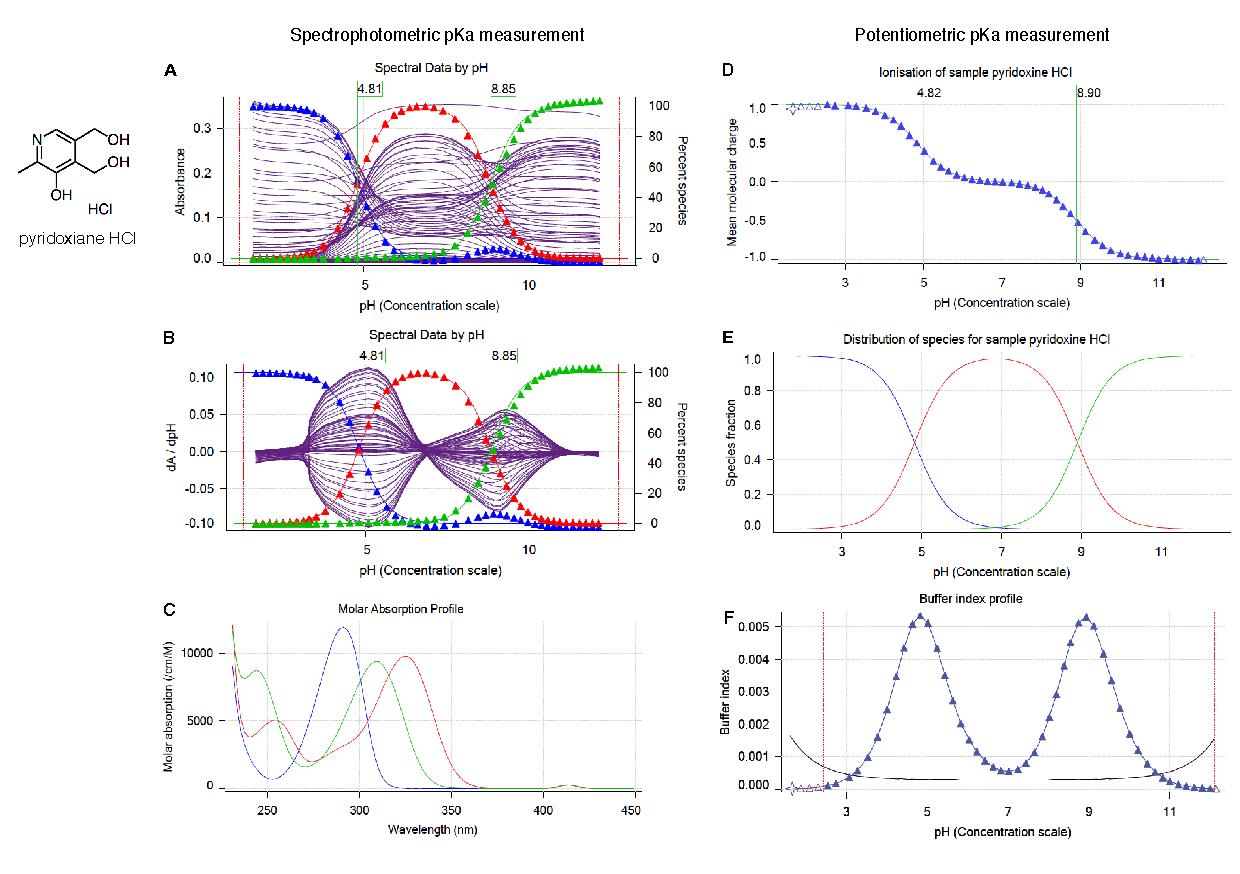
\includegraphics[width=0.95\linewidth]{figures/UVmetric_vs_pHmetric_pKa_figure}
\caption{{\bf Spectrophotometric (UV-metric) and potentiometric (pH-metric) pKa measurements of pyridoxine HCl with Sirius T3.} Spectrophotometic method (panels \textbf{A, B, C}) relies on UV-absorbance difference between protonation states.  It is very sensitive and requires very low analyte concentrations($\sim$ 50~\micro M), but limited to titration sites near chromophores. \textbf{A} Multiwavelength absorbance vs pH. Purple lines represents absorbance at each wavelength in UV-region.  \textbf{B} Derivative of multiwavelength absorbance with respect to pH (dA/dpH) vs pH is plotted with purple lines. In \textbf{A} and \textbf{B} Blue, red, and green triangles represent population of protonation states calculated from experimental data at each pH value. pKa values (green flags) correspond to inflection point of multiwavelength absorbance data where change in absorbance with respect to pH is maximum. \textbf{C} Molar absorption coefficients vs wavelength for each protonation state as resolved by TFA. \textbf{D, E, F} illustrate potentiometric pKa measurement where molar addition of acid or base is tracked as pH is titrated.\textbf{D} Mean molecular charge vs pH. Mean molecular charge is calculated based on the model provided for the analyte: predicted number and nature of titratble sites(acid or base type), and number of counter ions present. pKa values are calculated as inflection points of charge vs pH plot. \textbf{E} Predicted macroscopic protonation state populations vs pH calculated based on pKa values (\ce{H2A+}: blue, \ce{HA}: green, and \ce{A-}) \textbf{E} Buffering index vs pH profile of water (grey solid line, theoretical) and the sample solution (blue triangles represent experimental data points). A higher concentration of analyte ($\sim$ 5~mM) is necessary for potentiometric method than for spectrophotometric method to provide large enough buffering capacity signal above water for an accurate measurement. 
}
\label{fig:fullwidth}
\end{figure}

\todo[inline]{Brief outline of what this paper includes.}

%%%%%%%%%%%%%%%%%%%%%%%%%%%%%%%%%%%%%%%%%%%%%%%%%%%%%%%%%%%%
% Methods
%%%%%%%%%%%%%%%%%%%%%%%%%%%%%%%%%%%%%%%%%%%%%%%%%%%%%%%%%%%%
\section{Methods}

\subsection{Compound selection and procurement}
Small molecules were purchased in powder form.
\todo[inline]{FIGURE for compound filtering steps. Flow chart or funnel for Illustration of compound selection and experimental measurement workflow.}
\todo[inline]{SI TABLE vendor, lot numbers, SMILES. Selected compounds and their SAMPL challenge identities, eMolecules ID, supplier reported purity, LC/MS purity}
\todo[inline]{FIGURE compound structures with pKa values + SEM}


\subsection{UV-metric pKa measurements}

Experimental pKa measurements were collected using spectrophotometric pKa method with a Sirius T3 automated titrator instrument (Pion) at 25°C and constant ionic strength. Sirius T3 instrument is equiped with an Ag/AgCl double-junction reference electrode to monitor pH, a dip probe attached to spectrophotometer that measures, a stirrer, and automated volumetric titration capability. The UV-metric pKa measurement protocol of the Sirius T3 measures the change in multiwavelength absorbance in the 250-450 nm UV region of the absorbance spectrum while the pH is titrated between pH 1.8 and 12.2 to evaluate pKas~\citep{tam_multi-wavelength_2001, allen_multiwavelength_1998}. 

10~mg/ml DMSO solutions of each compound were prepared by weighing 1 mg of powder chemical with Sartorius Analytical Balance (Model: ME235P) and dissolving it in 100~\micro L DMSO (Dimethyl sulfoxide, Fisher Bioreagents, CAT: BP231-100, LOT: 116070, purity $\geq$ 99.7\%).  DMSO stock solutions were capped immediately to limit hygroscopicity of DMSO and sonicated for 5-10 minutes in water bath sonicator at room temperature to ensure proper dissolution. These DMSO stock solutions were stored in room temperature up to 2 weeks. 10~mg/ml DMSO solutions were used as stock solutions for the preparation of 3 replicate samples for independent titrations:  1\-5 \micro L of 10~mg/ml DMSO stock solution delivered to 4~mL glass sample vials of Sirius T3 with an electronic micropipette (Rainin EDP3 LTS 1-10 \micro L). The volume of delivered DMSO stock solution, which determines the sample concentration, is optimized individually for each compound to achieve sufficient but not saturated absorbance signal (targeting 0.5-1.0 AU) in the linear response region. Another limiting factor for sample concentration was ensuring that the compounds stays soluble in the whole range of pH titration range. 25~\micro L of mid-range buffer (14.7~mM \ce{K2HPO4} 0.15 M \ce{KCl} in \ce{H2O}) was added to each sample transfered with a micropipette (Rainin EDP3 LTS 10-100 \micro L)) to provide enough buffering capacity in middle pH ranges so that pH could be controlled incrementally throughout the titration.  

pH is temperature and ionic\textendash strength dependent. Sample heating block of Sirius T3 kept the analyte solution at $25 \pm 1$~\textdegree C throughout the titration. Ionic\textendash strength of the samples were adjusted by dilution in 1.5 mL ionic\textendash strength adjusted water (ISA water, 0.15~M KCl) to the vials by Sirius T3.  Analyte dilution, mixing, acid/base titration, and measurement of UV-absorbance was automated by UV-metric pKa measurement protocol of Sirius T3(Pion). pH was titrated between pH 1.8 and 12.2 with addition of acid (0.5~M HCl) and base (0.5~M KOH) targeting 0.2 pH steps between datapoints. Titrations were performed under Argon flow on the surface of sample solution to limit carbondioxide absorption from air. To capture all sources of experimental variability fully, instead of doing 3 tandem pH titrations on the same sample solution, pKas of three replicate samples were measured separately with one round of pH titration. Although this choice has higher cost for throughput and analyte consumption, it limits the dilution of the analyte during multiple titrations and drop in absorbance signal. 

Visual inspection of sample solutions after titration and inspection of pH-dependent absorbance shift in 500-600 nm region of UV spectra was used to verify no detectable precipitation occurred during the course of measurement. Absorbance in 500-600 nm region of UV spectra is associated with scattering of longer wavelengths of light in the presence of aggregates. For each analyte, we optimized analyte concentration, direction of titration and the range of pH titration in order to achieve solubility. The direction of titration was determined so that titration would start from the pH where the compound is most soluble: low-to-high pH for bases and high-to-low pH for acids. UV-metric pKa measurement method typically requires as low as 50~\micro M sample concentration (although minimum concentration requirement may change based on absorbance properties of the analyte). Some compounds may not be solube even at such low concentration throughout pH range of the titration. As the sample is titrated through a wide range of pH values, it is likely that low solubility ionization states such as neutral and zwitterionic states will be also be visited, limiting the highest analyte concentration that can be titrated without encountering any solubility issues.  For compounds with insufficient solubility to accurately determine a pKa directly in a UV-metric titration, a cosolvent protocol was used [See the next section: UV-metric pKa measurement with cosolvent]. 

The Sirius T3 software \todo{Add software name and version} was used to execute measurement protocols and to analyze pH-dependent multivelenghth spectra.
A protonation state change of titratable sites near chromophores will modulate the UV-absorbance spectra of these chromophores, allowing populations of distinct UV-active species to be resolved as a function of pH. To do this, basis spectra are identified and populations extracted via TFA analysis of the pH-dependent multi-wavelength absorbance ~\citep{allen_multiwavelength_1998}. When fitting the absorbance data to a titratable molecule model to estimate pKas, we selected the minimum number of pKas that was sufficient to provide a high quality of fit between experimental and modeled data based on visual inspection of pH-dependent populations.

This method is capable of measuring pKas between 2 and 12 when protonatable groups are at most 4-5 heavy atoms away from chromophores such that a change in protonation state alters the absorbance spectrum of the chromophore. We have selected compounds where titratable groups are close to potential chromophores (generally aromatic ring systems), but it is possible that our experimental results couldn't detect protonation of titratable groups distal to a UV-chromophore.

\todo[inline]{FIGURE: how potentiometric and UV-metric data looks side by side. Example UV-metric titration and data analysis.}


\subsection{UV-metric pKa measurement with cosolvent}
If analytes are not sufficiently soluble in aqueous environment, pKa values can not be determined accurately with UV-metric pKa measurements method. If precipitation is present, the UV-absobance signal from pH-dependent precipitate formation can not be differentiated from the pH-dependent protonation signal. For compounds with low aqueous solubility pKa values were estimated from multiple apparent pKas measurements done in methanol:water cosolvent solutions with various ratios. This method is refered to as UV-metric psKa method in Sirius T3 Manual ~\citep{noauthor_sirius_2008}.

In cosolvent spectrophotometric pKa measurement protocol was very similar to UV-metric pKa measurement method in water except the following aspects: Three titrations were performed in typically in 30\%, 40\%, and 50\% mixtures methanol:water by volume to measure apparent pKa values (psKa) in these mixtures. Than Yasuda-Shedlovsky extrapolation method was used to estimate the pKa value at 0\% cosolvent~\citep{avdeef_ph-metric_1999,doi:10.1021/ac00049a010,TAKACSNOVAK1997235}. 

$$ psKa + log [\ce{H2O}]=A/\epsilon+B $$
Yasuda-Shedlovsky extrapolation relies on the linear correlation between $psKa + log [\ce{H2O}]$ and reciprocal dielectric constant of the cosolvent mixture ($1/\epsilon$). In the equation above, A and B are the slope and intercept of the line fitted to experimental datapoints.  Depending on the solubility requirements of the analyte methanol ratio of the cosolvent mixtures were adjusted. Calculation of Yasuda-Shedlovsky extrapolation was performed by Sirius T3 software using at least 3 psKa values measured in different ratios of methanol:water.
Addition of methanol (ISA, 0.15 M KCl) was controlled by the instrument before each titration. Three consecutive pH titrations at different methanol concentrations were performed using the same sample solution. In addition, three replicate measurements with independent samples (prepared from the same DMSO stock) were collected.

\todo[inline]{FIGURE: EXTRAPOLATION}

\subsection{Calculation of uncertainty in pKa measurements}
Experimental uncertainties were reported as standard error of the mean (SEM) of three replicate pKa measurements. Since Sirius T3 software reports pKa values with 2 decimal places, we have reported SEM as 0.01 in cases where SEM values calculated from 3 replicates were lower than 0.01.


\subsection{Protonation site determination with NMR}
\todo[inline]{Update or remove this section based on updates from Iyke.}

\subsection{Quality control for chemicals}
Purity of SAMPL6 pKa challenge compounds were determined based on LC\textendash MS. The purity analysis was performed using an Agilent HPLC1200 Series equipped with auto\textendash  sampler, UV diode array detector and a Quadrupole MS detector 6140. The software used was Chemistation for LC \& LC\/MS with version C01.07SR2.
The column for the analysis is Assentis Express C18 3.0x100mm 2.7~µl particle size at Column temperature~=~45\textdegree C.
\begin{itemize}

\item Mobile phase A: 2~mM ammonium formate ( pH=3.5) aqueous
\item Mobile phase B: 2~mM ammonium formate in Acetonitrile : Water=90:10 ( pH=3.5)
\item Flow rate : 0.75ml/min
\item Gradient: Starting with 10\% B to 95\%B in 10 minutes then hold 95\%B for 5 minutes. 
\item Post run length: 5 minutes 
\item Mass condition: ESI positive and negative mode
\item Capillary voltage: 3000~V
\item Grying gas flow: 12~ml/min
\item Nebulizer pressure: 35~psi
\item Drying temperature: 350\textdegree C
\item Mass range: 5-1350~Da; Fraggmentor:70; Threshold:100
\end{itemize}

The percent area for main peak is calculated based on the area of main peak divided by the total area of all peaks. The percent area of the main peak is reported as an estimate of sample purity.

\todo[inline]{SI Figure: all MS data}

%%%%%%%%%%%%%%%%%%%%%%%%%%%%%%%%%%%%%%%%%%%%%%%%%%%%%%%%%%%%
% Results
%%%%%%%%%%%%%%%%%%%%%%%%%%%%%%%%%%%%%%%%%%%%%%%%%%%%%%%%%%%%
\section{Results}

\begin{figure}
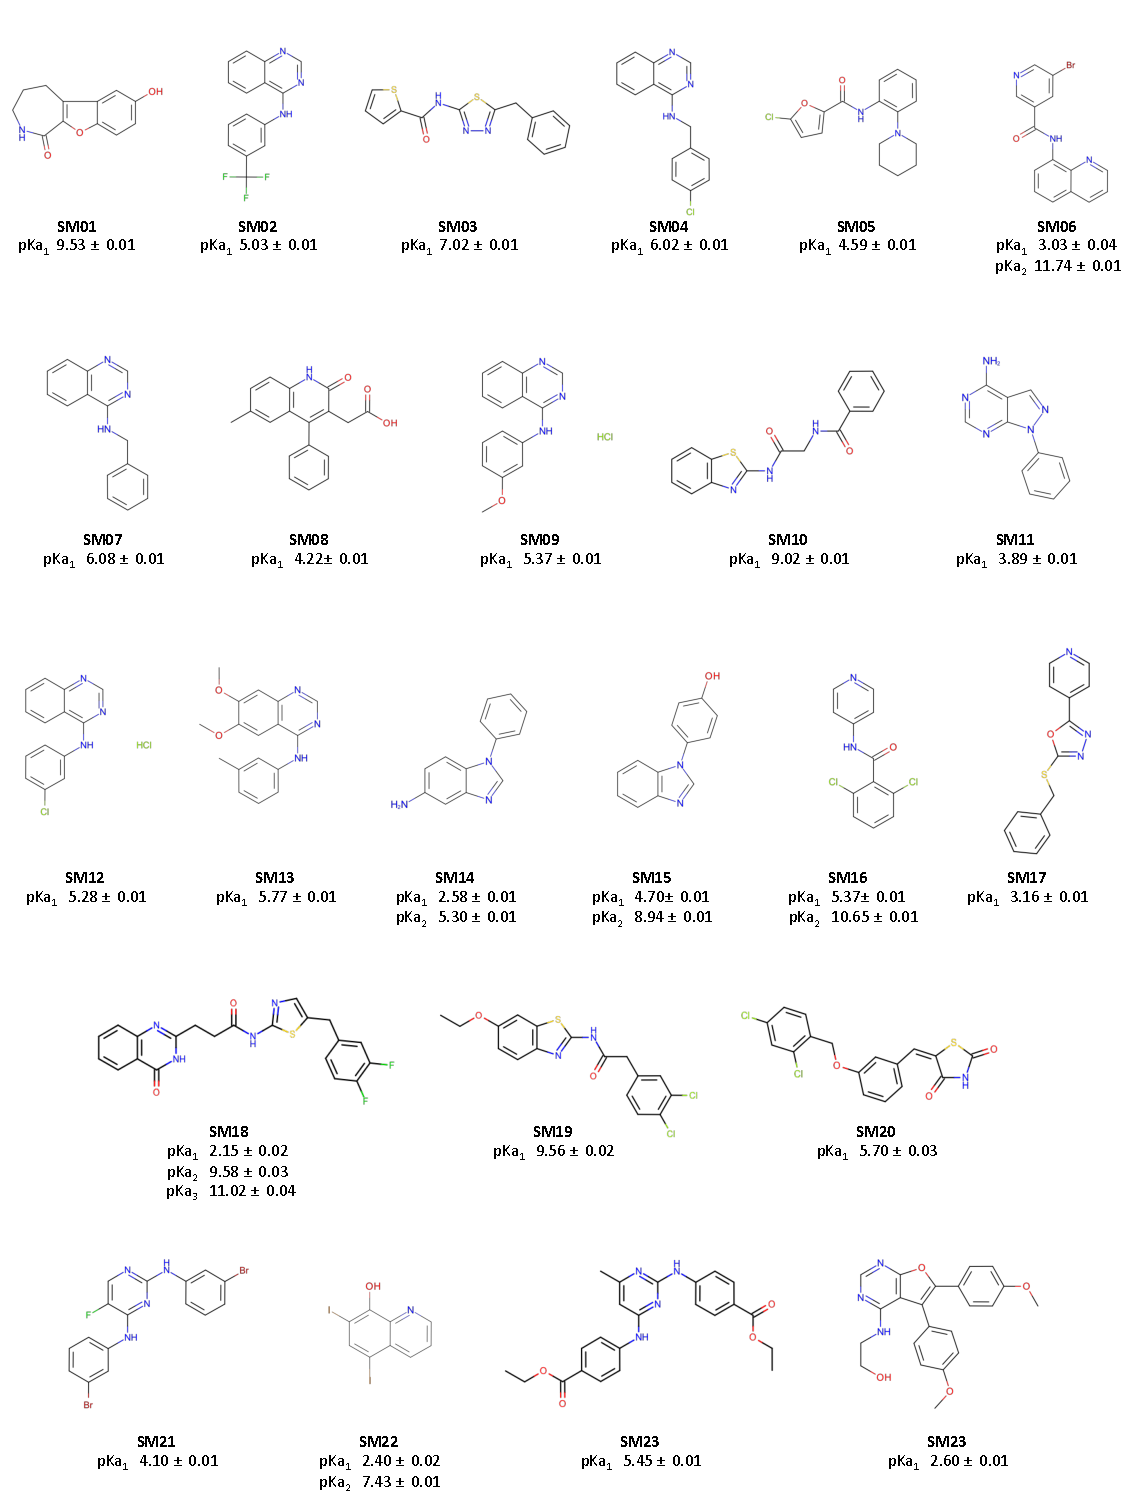
\includegraphics[width=0.95\linewidth]{figures/SAMPL6_pKa_molecules_fig}
\caption{{\bf Molecules used in the SAMPL6 \pKa  challenge.} 
Experimental UV-metric \pKa measurements were performed for these 24 molecules, and discernable macroscopic {\pKa}s reported. 
Uncertainties are expressed as the standard error of the mean of three independent measurements.
}
\label{fig:fullwidth}
\end{figure}


\todo[inline]{TABLE:  Measured macroscopic pKa for all compounds, what method}
\todo[inline]{Effect of cosolvent on measured pKas}
\todo[inline]{FIGURE: Cosolvent vs non-cosolvent measurement difference}

%%%%%%%%%%%%%%%%%%%%%%%%%%%%%%%%%%%%%%%%%%%%%%%%%%%%%%%%%%%%
% Discussion
%%%%%%%%%%%%%%%%%%%%%%%%%%%%%%%%%%%%%%%%%%%%%%%%%%%%%%%%%%%%
\section{Discussion}
\todo[inline]{Discussion of experimental data interpretation: macroscopic}
Multiwavelength absorbance analysis on thw Sirius T3 allows for very good resolution of pKas, but it is important to note that this method produces estimates of macroscopic pKas. If multiple microscopic pKas have close pKa values and overlapping changes in UV absorbance spectra associated with protonation/deprotonaton event, the spectral analysis could produce a single macroscopic pKa that represents an aggregation of multiple microscopic pKas.
\todo[inline]{Warning about acid base assingment from cosolvent measurements}
\todo[inline]{Lessons learned for future challenge iterations}
\todo[inline]{Challenges with NMR measurments?}
\todo[inline]{pKa can shift based on ionic strength, temperature, and lipophilic content
Can other cosolvents be interesting for process chemistry.}

%%%%%%%%%%%%%%%%%%%%%%%%%%%%%%%%%%%%%%%%%%%%%%%%%%%%%%%%%%%%
% Code and Data Availability
%%%%%%%%%%%%%%%%%%%%%%%%%%%%%%%%%%%%%%%%%%%%%%%%%%%%%%%%%%%%
\section{Code and data availability}
\begin{minipage}{15cm}
\begin{itemize}
%\item Compound selection scripts are available at \href{https://github.com/}{https://github.com/} under \"compound_selection\" directory.
% https://github.com/choderalab/sampl6-physicochemical-properties

\item SAMPL6 pKa challenge instructions, submissions, and analysis is available at  \href{https://github.com/MobleyLab/SAMPL6}{https://github.com/MobleyLab/SAMPL6}

\item Python scripts used for compound selection are available at \textbf{compound\textunderscore selection} directory of  
\href{https://github.com/choderalab/sampl6\textendash physicochemical\textendash properties}{https://github.com/choderalab/sampl6-physicochemical-properties}

\end{itemize}
\end{minipage}



\todo[inline]{Construct a proper README for compound selection directory.}
%%%%%%%%%%%%%%%%%%%%%%%%%%%%%%%%%%%%%%%%%%%%%%%%%%%%%%%%%%%%
% Overview of supplementary information
%%%%%%%%%%%%%%%%%%%%%%%%%%%%%%%%%%%%%%%%%%%%%%%%%%%%%%%%%%%%
\section{Overview of supplementary information}

%%%%%%%%%%%%%%%%%%%%%%%%%%%%%%%%%%%%%%%%%%%%%%%%%%%%%%%%%%%%
% Author Contributions 
%%%%%%%%%%%%%%%%%%%%%%%%%%%%%%%%%%%%%%%%%%%%%%%%%%%%%%%%%%%%
\section{Author Contributions}
\todo[inline]{Complete this section.}

Conceptualization, ; Methodology, ; Software, ; Formal Analysis, ; Investigation, MI, ; Resources, ;  Data Curation, ; Writing-Original Draft, ; Writing - Review and Editing, ; Visualization, ; Supervision, ; Project Administration, ; Funding Acquisition, 

%(Follow the \href{http://www.cell.com/pb/assets/raw/shared/guidelines/CRediT-taxonomy.pdf}{CRediT Taxonomy})

%%%%%%%%%%%%%%%%%%%%%%%%%%%%%%%%%%%%%%%%%%%%%%%%%%%%%%%%%%%%
% Acknowledgments 
%%%%%%%%%%%%%%%%%%%%%%%%%%%%%%%%%%%%%%%%%%%%%%%%%%%%%%%%%%%%
\section{Acknowledgments}
\todo[inline]{Complete this section.}

MI, ASR, and JDC acknowledge support from the Sloan Kettering Institute. JDC acknowledges support from NIH grant P30 CA008748. MI acknowledges Doris J. Hutchinson Fellowship. Acknowledging Merck Preformulation department for materials, expertise and instrument time.

Brad Sherborne  
Paul Czodrowski - helped with purchasable compound list in earlier iteration  
Ikenna Ndukwe  
Caitlin Bannan  

%%%%%%%%%%%%%%%%%%%%%%%%%%%%%%%%%%%%%%%%%%%%%%%%%%%%%%%%%%%%
% Disclosures 
%%%%%%%%%%%%%%%%%%%%%%%%%%%%%%%%%%%%%%%%%%%%%%%%%%%%%%%%%%%%
\section{Disclosures}

JDC is a member of the Scientific Advisory Board for Schr\"{o}dinger, LLC.

\nocite{*} % This command displays all refs in the bib file. PLEASE DELETE IT BEFORE YOU SUBMIT YOUR MANUSCRIPT!
\bibliography{elife-sample}

%%%%%%%%%%%%%%%%%%%%%%%%%%%%%%%%%%%%%%%%%%%%%%%%%%%%%%%%%%%%
% Supplementary Information
%%%%%%%%%%%%%%%%%%%%%%%%%%%%%%%%%%%%%%%%%%%%%%%%%%%%%%%%%%%%
\newpage
\section{Supplementary Information}









\end{document}
